\section{理论框架}
项目的理论框架主要包括当前行人重识别领域state-of-the-art的算法思想、摄像头部署方案的评价指标以及强化学习模型在项目中的应用。

\subsection{行人重识别领域state-of-the-art的算法思想}

\subsubsection{Part-based Convolutional Baseline (PCB)}
这篇论文的Baseline采用了最近很热门的Part的思想,但不同于计算图片中的Attention,而是简单地将图片在垂直方向上分块,获取每一个块的特征。

图\ref{fig:baseline} 是Baseline的架构图。在Baseline中,模型以ResNet50作为Backbone Network。ResNet50模型首先在ImageNet数据集上训练至收敛,然后去掉为ImageNet分类任务而设计的全局池化层(Global Average Pooling Layer)及其后面的全连接层(Fully Connected Layer),使ResNet50模型成为一个高效的图像特征提取器,其中的特征既包括颜色、纹理、形状等视觉特征,也包括类别、姿势、性别等语义特征。作为一个端到端(End-to-End)的特征提取器,其输入为包含RGB通道的原始图像,输出为包含2048个通道(2048 Channels)的Feature Maps。

将ResNet50模型输出的Feature Maps在竖直方向上分成$p=6$个水平条(Horizontal Stripes),每个通道(Channel)保持独立。每个水平条通过一个尺寸与水平条尺寸相同全局池化层,使得原本为矩形的水平条变为一个$1\times1$的像素点,再将其与同一水平条其他通道的像素点拼接起来得到一个$2048\times1\times1$的向量。因为每个水平条会得到一个特征向量,所以经过全局池化层之后可得到$p$个向量,每一个向量都能表示原图像在对应的水平条范围内的局部特征。此方法的优点是简单、高效、易实现,缺点是每个人各部位的分布不同,人物上所具备的关注点也千差万别,将Feature Maps在竖直方向上均匀分割不能很好地体现人与人之间的这些差异。

得到$p$个2048维的特征向量之后,再使用核尺寸为$1\times1$的卷积层将每个2048维的向量降为256维,以减少之后分类任务的计算量。每一个局部特征向量后接一个$n$分类器以预测该图像的类别,其中$n$为训练集中label的个数。训练的损失函数(Loss Function)使用交叉熵损失(Cross Entropy Loss)。

在测试阶段,也即特征提取阶段,将最后的$p$个$n$分类器去掉,直接将$p$个256维的向量拼接(concatenate)为向量$\textbf g$或将$p$个2048维的向量拼接为向量$\textbf h$作为原始行人图像的特征表示。

\subsubsection{Refined Part Pooling (RPP)}
Part-based Convolutional Baseline (PCB) 将Feature Maps在竖直方向上均匀分成$p$个水平条,以获得行人各部位的特征。此方法有操作简单、运算量少、易于实现的优点,但忽略了人与人之间各部位的位置差距。因此,有必要在Baseline的基础上进行改进,不再局限于一个规范的矩形,而是通过计算判断每一个像素点「应该属于」哪一个部分。如图\ref{fig:refined}所示。对于不同通道、相同位置的像素点,进行统一处理。

于是目标就成了:给定一个列向量(column vector,表示不同通道、相同位置的像素点),判断其属于哪一个部分。这就变成了一个分类问题。在这里使用一个线性神经网络层,来将所有的列向量分类。线性神经网络层有权重$W$和偏置$b$组成,为了简化表示,这里省略偏置$b$。对于一个列向量$f$,其属于第$i$个部分的概率$P(p_i|f)$为:
\begin{equation}
P(p_i|f)=\mathop{\rm softmax}\left(W_i^{\rm T}f\right)=\frac{\exp\left(W_i^{\rm T}f\right)}{\sum_j^p\exp\left(W_j^{\rm T}f\right)}
\end{equation}
其中$p_i$表示Feature Map的第$i$部分。

在PCB中,列向量$f$只绝对的属于某一个部分。在求得$P(p_i|f)$后,则可将原始的列向量$f$按照概率分布分配到各部分。对于第$i$个部分$p_i$,其计算方式为:
\begin{equation}
p_i=\frac{1}{H\times W}\sum_{j=1}^{H\times W}P(p_i|f_j)\times f_j
\end{equation}
其中$H$、$W$分别代表Feature Map的高和宽。

如此一来即可得到与PCB算法等价的输出,再经过与PCB算法后半部分相同的$1\times1$卷积层和分类器,便完成了Refined Part Pooling (RPP)算法的训练模型。完整的PCB+RPP架构图如图\ref{fig:structure2}所示。

\begin{figure}
\centering
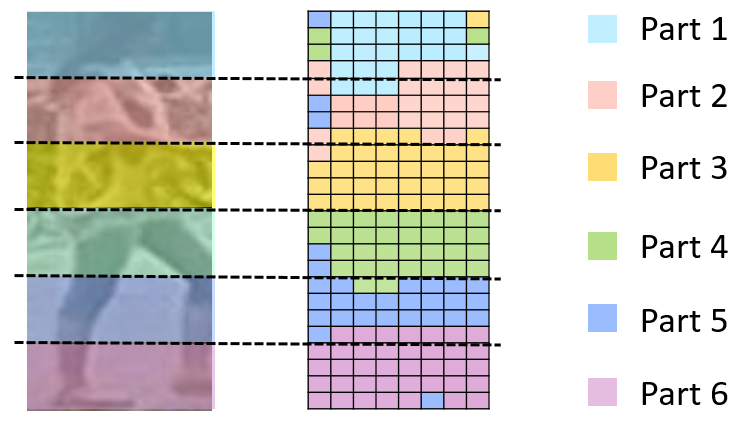
\includegraphics[width=0.6\textwidth]{figure/outliers1}
\caption{Refined Part Pooling示意图}
\label{fig:refined}
\end{figure}

\subsection{监控摄像头部署方案的评价指标}

监控摄像头的部署方案包括摄像头的数量以及部署位置。摄像头的部署位置会影响监控场景的完整性、监控画面的光线质量以及监控目标的呈现角度。而监控摄像头数量受成本预算的限制,不可能无限增加,因此在预算有限的约束下,如何设计监控摄像头的部署位置,使得监控效果最优,便成为一个值得研究的问题。而在研究优化问题之前,需要定义监控摄像头部署方案的评价指标。

监控效果的优劣可以定义为在当前的监控方案下,跨摄像头追踪特定行人的能力。当前在多摄像头多行人追踪(Multi-Target Multi-Camera Tracking,Multi-Target Multi-Camera Tracking)领域主流的评价指标有多目标跟踪准确度(MOTA)和识别F值(IDF1)。

\subsubsection{多目标跟踪准确度(MOTA)}

多目标跟踪准确度(Multiple Object Tracking Accuracy,MOTA)

\subsubsection{识别F值(IDF1)}

识别F值(Identification F-Score,IDF1)

\subsection{强化学习模型}

\subsection{面向CPU集群的分布式深度学习训练框架}

\begin{figure}
\centering
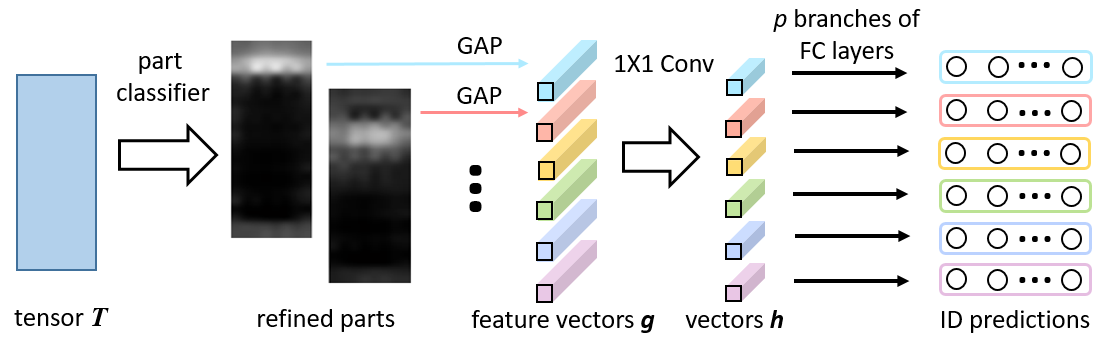
\includegraphics[width=1\textwidth]{figure/structure2}
\caption{PCB+RPP架构图}
\label{fig:structure2}
\end{figure}